\documentclass[a4paper,10pt]{article}

% ---------- Fonts and page layout ----------
% （注）フォント名は本環境（macOS + Tectonic）で解決できる表記に合わせ，
%  phase2 レポートの TeXGyreTermes / TeXGyreHeros をスペース入り正式名で指定している。
\usepackage{xeCJK}
\setmainfont{TeX Gyre Termes}
\setsansfont{TeX Gyre Heros}
\setmonofont{DejaVu Sans Mono}
\setCJKmainfont{Noto Serif CJK JP}
\setCJKsansfont{Noto Sans CJK JP}
\setCJKmonofont{Noto Sans Mono CJK JP}
\XeTeXlinebreaklocale "ja"
\XeTeXlinebreakskip=0pt plus 1pt

\usepackage[a4paper,left=24mm,right=24mm,top=24mm,bottom=25mm]{geometry}
\usepackage{setspace}
\setstretch{1.15}
\setlength{\parindent}{1em}
\setlength{\parskip}{0.25em}

% ---------- Math, tables, figures ----------
\usepackage{amsmath,amssymb,mathtools}
\usepackage{graphicx}
\usepackage{booktabs}
\usepackage{longtable}
\usepackage{tabularx}
\usepackage{array}
\usepackage{multirow}
\usepackage{makecell}
\usepackage{float}
\usepackage{caption}
\usepackage{xcolor}
\usepackage{enumitem}
\usepackage{titlesec}
\usepackage{fancyhdr}
\usepackage[hidelinks]{hyperref}
\usepackage{url}
\usepackage{microtype}
\usepackage[most]{tcolorbox}

\graphicspath{{figures/}}

% ---------- Unified style ----------
\definecolor{bbblack}{HTML}{222222}
\definecolor{bbgray}{HTML}{666666}
\definecolor{bblight}{HTML}{F2F2F2}
\definecolor{bbline}{HTML}{333333}
\renewcommand{\figurename}{Figure}
\renewcommand{\tablename}{Table}
\captionsetup{font={small},labelfont={bf},justification=raggedright,singlelinecheck=false}
\captionsetup[table]{position=top}
\captionsetup[figure]{position=bottom}
\renewcommand{\arraystretch}{1.22}
\setlist[itemize]{leftmargin=1.6em,itemsep=0.15em,topsep=0.2em}
\setlist[enumerate]{leftmargin=1.8em,itemsep=0.15em,topsep=0.2em}

\titleformat{\section}{\sffamily\bfseries\Large\color{bbblack}}{\thesection}{0.8em}{}
\titleformat{\subsection}{\sffamily\bfseries\large\color{bbblack}}{\thesubsection}{0.7em}{}
\titleformat{\subsubsection}{\sffamily\bfseries\normalsize\color{bbblack}}{\thesubsubsection}{0.6em}{}
\titlespacing*{\section}{0pt}{1.2em}{0.5em}
\titlespacing*{\subsection}{0pt}{0.9em}{0.35em}
\titlespacing*{\subsubsection}{0pt}{0.7em}{0.25em}

\pagestyle{fancy}
\fancyhf{}
\lhead{\small\sffamily BEYOND BUFFETT Phase3 Methodology}
\rhead{\small\sffamily 離：Moatの時間軸拡張}
\cfoot{\small\thepage}
\renewcommand{\headrulewidth}{0.4pt}

\newcolumntype{Y}{>{\raggedright\arraybackslash}X}
\newcommand{\metric}[1]{\mathrm{#1}}
\newcommand{\ind}[1]{\mathbf{1}\{#1\}}

\newtcolorbox{keybox}[1][]{
  colback=bblight, colframe=bblight, boxrule=0pt, arc=1mm,
  left=2mm, right=2mm, top=2mm, bottom=2mm, breakable,
  before skip=6pt, after skip=6pt,
  title={#1}, coltitle=bbblack, fonttitle=\sffamily\bfseries,
  attach title to upper={\par}
}
\newtcolorbox{defbox}[1][直感]{
  colback=white, colframe=bbline, boxrule=0.6pt, arc=1mm,
  left=2mm, right=2mm, top=2mm, bottom=2mm, breakable,
  before skip=6pt, after skip=6pt,
  title={#1}, coltitle=bbblack, fonttitle=\sffamily\bfseries,
  attach title to upper={\par}
}

\begin{document}

% ---------- Cover ----------
\begin{titlepage}
\centering
\vspace*{12mm}
{\sffamily\bfseries\Huge BEYOND BUFFETT\par}
\vspace{6mm}
{\sffamily\bfseries\LARGE Phase3 解説レポート\par}
\vspace{3mm}
{\sffamily\Large 離：変わる堀・生まれる堀を測り，最終20社を組む\par}
\vspace{14mm}
{\large 本資料は，Phase2 で形成した候補宇宙 Top1200 から，\par}
{\large 「変わる Moat」「生まれる Moat」を証拠水準つきで測定し，\par}
{\large 三世代の堀からなる最終 20 社を構成するまでを，0 から解説する。\par}
\vfill
{\small 正典データ：phase3\_moat\_construction／phase3\_beyond\_buffett\_v2\par}
\end{titlepage}

\setcounter{tocdepth}{2}
\tableofcontents
\clearpage

% ---------- 1 ----------
\section{エグゼクティブサマリー}

Phase3 の目的は，AI テーマ株を集めることでも，低 PBR 株を集めることでもない。Phase1（守）が抽出した「完成した堀」に，これから資本効率改革で「変わる堀」と，産業構造の転換から「生まれる堀」を加え，三世代の堀からなる 20 社を，反証可能な形で構成することである。

\begin{keybox}[Phase3 の一文定義]
\centering
\Large 堀を時間軸で三世代に広げ，証拠で裏づけて 20 社に束ねる。
\end{keybox}

この一文を式と手続きへ分解すると，表\ref{tab:p3-map}のようになる。

\begin{table}[H]
\caption{Phase3 で用いる考え方と式の対応}
\label{tab:p3-map}
\centering
\small
\begin{tabularx}{\linewidth}{p{34mm}Y p{44mm}}
\toprule
投資上の問い & 定量化する概念 & 使用する主な式 \\
\midrule
これから変わるか & Transformation Moat & 式\eqref{eq:trans-partial}（partial 実装形） \\
これから生まれるか & Emerging Moat & 式\eqref{eq:emerging} \\
根拠はどれだけ具体的か & Evidence Level & 式\eqref{eq:evidence} \\
どう束ねるか & 五役割の設計 & 5/5/5/3/2（\ref{sec:roles}節） \\
壊れていないか & 感度・除外監査 & $\pm20\%$ 感度・862社の理由別記録 \\
\bottomrule
\end{tabularx}
\end{table}

重要なのは三点である。第一に，Phase3 の独自性は新式の発明ではなく，Phase1 の先行研究部品（割安・改善・利益の質）を時間軸の方向へ再構成した点にある。第二に，設計上の完全形（式\eqref{eq:trans-design}）と実際に選定へ使った実装形（式\eqref{eq:trans-partial}）を峻別し，完全形を使ったかのように書かない。第三に，スコアの高さと証拠の強さを混同しないため，Evidence Level をスコアから分離して管理する。最終 20 社の分布は Level 3 が 15 社，Level 2 が 4 社，Level 1 が 1 社である。

\section{この資料の読み方：0から理解するための順序}

本資料は，簿記・投資の前提知識がない読者を想定し，次の順で読めるように構成した。まず\ref{sec:why}節で，なぜ完成した堀だけでは足りないのかを確認する。次に\ref{sec:trans}節と\ref{sec:emerg}節で，変わる堀・生まれる堀をそれぞれ 0 から定義し，式に落とす。\ref{sec:evidence}節で証拠水準を分離し，\ref{sec:roles}節で 20 社の束ね方を示す。最後に，除外の監査（\ref{sec:rejected}節），頑健性（\ref{sec:robust}節），計算例（\ref{sec:example}節），限界（\ref{sec:limits}節）で締める。

\subsection{選定式と検証式を分ける}

Phase1・2 と同じく，本資料でも「選定に使った式」と「あとで確認に使った式」を厳密に分ける。式\eqref{eq:trans-partial}・\eqref{eq:emerging}・\eqref{eq:evidence}は選定に使った。$\pm20\%$ 感度やアブレーション（Phase5 資料）は確認であり，これらで銘柄を入れ替えることはしていない。

% ---------- 3 ----------
\section{なぜ Phase3 が必要なのか}
\label{sec:why}

\subsection{守・破・離の中での Phase3}

Phase1（守）は先行研究式だけで完成した堀を Top5 に圧縮し，Phase2（破）は式を変えずに候補宇宙を Top1200 へ広げた。しかし Phase1 の物差しは，定義上「いま完成している」堀しか測れない。堀は静的ではない。資本効率改革で変わる堀があり，産業構造の転換から生まれる堀がある。Phase3（離）で初めて独自の物差しを導入するのは，独自性がどこで何を変えたかを，守・破に遡って検証できるようにするためである。

\begin{figure}[H]
\centering
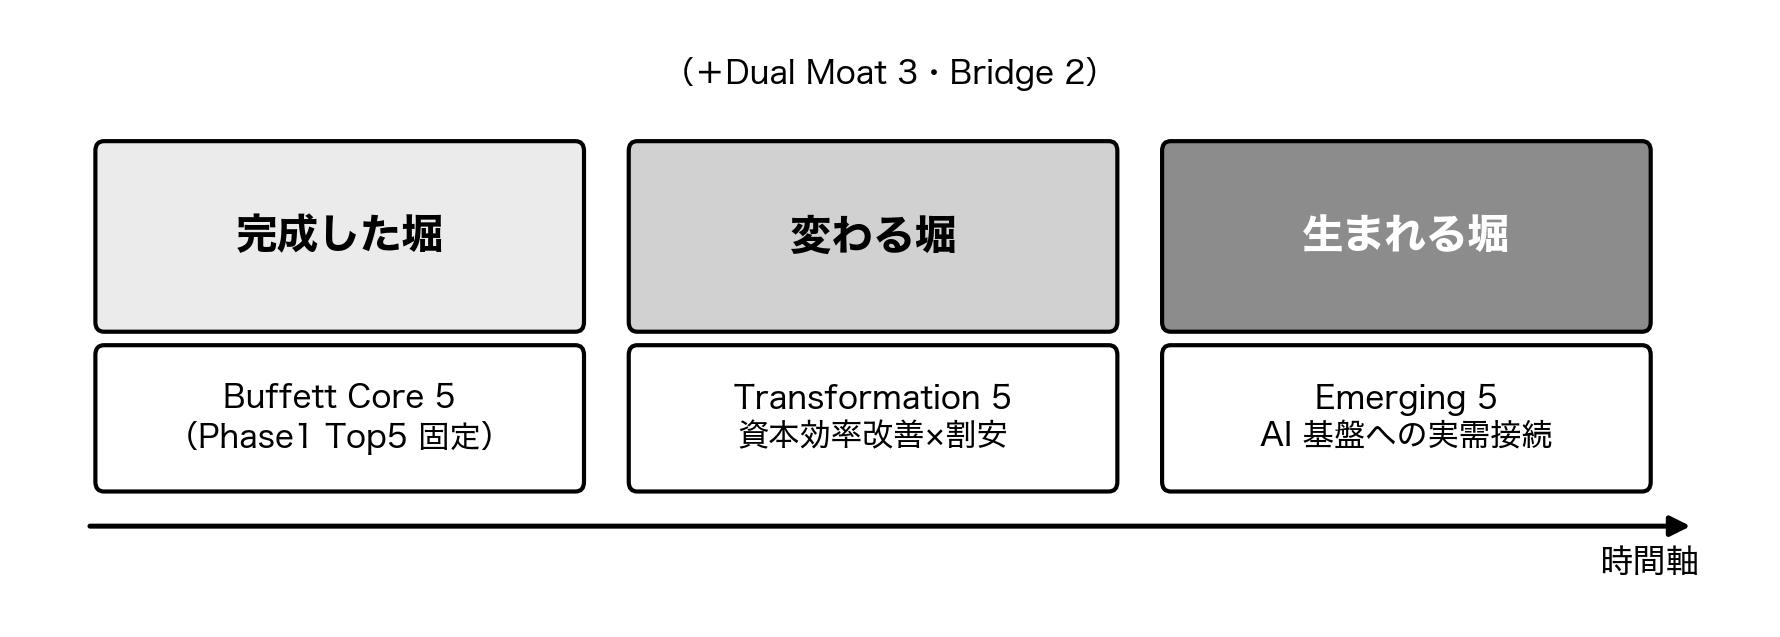
\includegraphics[width=0.9\linewidth]{p3_timeaxis.png}
\caption{三世代の堀。完成（Phase1 Top5 固定）・変化（Transformation）・新生（Emerging）に，両立型（Dual Moat）と分散役（Bridge）を加えて 20 社を構成する。}
\label{fig:timeaxis}
\end{figure}

\subsection{二つの地殻変動}

第一に，東京証券取引所（2023）の「資本コストや株価を意識した経営」要請である。伊藤レポート（経済産業省，2014）以来の資本収益性重視の流れが，PBR 1 倍割れ企業の経営改革を促し，長く割安に放置された企業の一部が実際に変わり始めた。第二に，生成 AI を起点とする構造転換である。半導体・光通信・データセンター・電力・品質保証といった基盤産業に実需の追い風が吹いている。ただし，開示資料で AI に言及するだけで具体的な製品・顧客・数量の裏づけを欠く企業は，本研究の調査で 577 社に上った。この二つを「テーマ買い」にせず式に落とすことが，Phase3 の課題である。

% ---------- 4 ----------
\section{変わる堀（Transformation Moat）を0から理解する}
\label{sec:trans}

\begin{keybox}[フローでの位置]
Transformation Score は，Top1200 のうち「割安だが，資本効率が実際に改善しており，還元の原資もある」企業を順位づけ，変わる堀 5 社（と両立型の一部）を選ぶために使う。低 PBR 株の選定ではない：割安でも定量的な改善証拠を欠く企業は「低 PBR のみ」として 15 社を除外した。
\end{keybox}

\subsection{バリュートラップとの違い}

株価が純資産に比べて安い（PBR が低い＝$\metric{BM}$ が高い）ことは，それだけでは買う理由にならない。安いのには理由があり，構造的に低収益のまま放置される企業は「割安のワナ（バリュートラップ）」と呼ばれる。変わる堀とは，割安であることに加えて，資本効率（ROA・ROE・マージン・回転率）の改善が実データで観測でき，株主還元の原資（フリーキャッシュフロー）があり，利益の質が健全な企業である。

\begin{defbox}
同じ PBR 0.7 倍でも，A 社は 3 年で ROA が改善し営業 CF が設備投資を上回るのに対し，B 社は赤字が続き改善の兆しがない。変わる堀の候補は A 社だけである。B 社は「低 PBR のみ」として除外される。
\end{defbox}

\subsection{設計完全形：何を測りたかったか}

設計段階では，変わる堀を六要素で測ることを意図した。

\begin{equation}
S^{\mathrm{Trans}}_i \;=\; 100\left(w_V V_i + w_C C_i + w_R R_i + w_E E_i + w_X X_i + w_Q Q_i\right) - P^{\mathrm{Trap}}_i.
\label{eq:trans-design}
\end{equation}

ここで $V_i$ は評価ギャップ，$C_i$ は資本効率改善，$R_i$ は株主還元，$E_i$ は改革開示，$X_i$ は実行信頼性，$Q_i$ は利益の質，$P^{\mathrm{Trap}}_i$ はバリュートラップ・ペナルティである。設計重みは $w_V{=}0.20$，$w_C{=}0.22$，$w_R{=}0.16$，$w_E{=}0.17$，$w_X{=}0.13$，$w_Q{=}0.12$ と置いた。

\textbf{ただし，この完全形は実際の銘柄選定には使っていない。}株主還元（$R$）と改革開示（$E$）の正式な構造化データが入力に存在しなかったためである。使えなかった式を使ったかのように書かないことは，本研究の誠実性の核である。

\subsection{partial 実装形：実際に使った式}

実際の選定には，入手できるデータだけで構成した次の partial 実装形を用いた。

\begin{equation}
S^{\mathrm{Trans,partial}}_i \;=\; 0.22\,V_i + 0.24\,C_i + 0.10\,F_i + 0.18\,X_i + 0.16\,Q_i + 0.10\,\Phi_i - P^{\mathrm{Trap}}_i.
\label{eq:trans-partial}
\end{equation}

設計形からの変更点は三つある。（i）株主還元 $R_i$ は，FCF プロキシ $F_i$（営業キャッシュフロー $-$ 設備投資が正なら還元余力ありとみなす）で代替した。（ii）改革開示 $E_i$ は除外した。なお改革開示レベル（TR）は Top1200 全社で同値となり識別力を持たなかったため，これを採用根拠に用いていない。（iii）Phase2 の分析信頼度 $\Phi_i$（0〜1.1）を加えた。値は $[0,100]$ にクリップする。スコア種別は，最終 20 社では partial が 19 社，lite（改善系列の一部欠損）が 1 社である。

\begin{table}[H]
\caption{式\eqref{eq:trans-partial}の部品と Phase1/2 由来}
\centering
\small
\begin{tabularx}{\linewidth}{p{30mm}Y p{42mm}}
\toprule
部品 & 内容 & 由来 \\
\midrule
$V_i$ 評価ギャップ & $\metric{BM}$・$\metric{EP}$ の正規化合成 & Fama--French／Basu（Phase1） \\
$C_i$ 資本効率改善 & ROA・ROE・マージン・回転率の 3 年変化 & Piotroski の改善思想の連続値化 \\
$F_i$ 還元余力 & $\metric{CFO}-\metric{CAPEX}>0$ & Sloan と同じ CF 系データ \\
$X_i$ 実行信頼性 & Piotroski available・CFO/NI & Phase1 \\
$Q_i$ 利益の質 & Sloan・distress 安全度 & Phase1 \\
$\Phi_i$ 信頼度 & Phase2 confidence & Phase2 \\
$P^{\mathrm{Trap}}_i$ & 高アクルーアル・営業CF赤字・継続損失 & Phase2 guardrail の再利用 \\
\bottomrule
\end{tabularx}
\end{table}

\subsection{ミニ演習：低 PBR だけの会社は残れるか}

$\metric{BM}=1.8$（強い割安）だが，3 年の ROA 改善がなく（$C_i$ 低），営業 CF が赤字（$P^{\mathrm{Trap}}$ 加点・$F_i=0$）の企業を考える。$V_i$ の寄与 0.22 だけでは合計は伸びず，ペナルティで押し下げられる。実際，この型の 15 社が「低 PBR のみ」として除外された。割安は入口にすぎず，改善の証拠が伴って初めて変わる堀になる。

% ---------- 5 ----------
\section{生まれる堀（Emerging Moat）を0から理解する}
\label{sec:emerg}

\begin{keybox}[フローでの位置]
Emerging Score は，AI・半導体・光通信・データセンター・電力・品質保証などの構造変化に「実需で」接続している企業を順位づけ，生まれる堀 5 社（と両立型の一部）を選ぶために使う。AI テーマ株の選定ではない：言及のみの 577 社はすべて除外し，理由を記録した。
\end{keybox}

\subsection{キーワードと堀を見分ける}

「AI に取り組む」と書くことは誰にでもできる。生まれる堀とは，構造変化の中で他社がまねしにくい位置（ボトルネック）を占め，それが売上・受注・投資額などの数量で裏づけられる状態を指す。たとえば光配線や超純水装置は，AI データセンターの建設に不可欠でありながら供給者が限られる。この「不可欠×希少」がボトルネック性である。

\subsection{Emerging Score の式}

\begin{equation}
S^{\mathrm{Emerg}}_i \;=\; 100\left(w_I I_i + w_N N_i + w_B B_i + w_A A_i + w_D D_i + w_T T_i\right) + B^{\mathrm{Evi}}_i - P^{\mathrm{Hype}}_i - P^{\mathrm{Guard}}_i.
\label{eq:emerging}
\end{equation}

$I_i$ は無形資産（R\&D 強度・粗利マージン力），$N_i$ は技術・イノベーション能力，$B_i$ はボトルネック性・価格決定力，$A_i$ は AI 産業基盤への接続，$D_i$ はデータ・顧客基盤，$T_i$ は信頼・安全基盤である。重みは $w_I{=}0.18,\ w_N{=}0.15,\ w_B{=}0.18,\ w_A{=}0.22,\ w_D{=}0.14,\ w_T{=}0.13$。証拠加点 $B^{\mathrm{Evi}}_i$ は最大 $+8$ に抑え，キーワードのみの言及には $P^{\mathrm{Hype}}_i=18$ 点の過熱ペナルティを課す。$P^{\mathrm{Guard}}_i$ は財務ガードレール罰である。値は $[0,100]$ にクリップする。

\begin{defbox}
証拠加点の上限（$+8$）を小さく，過熱ペナルティ（$18$）を大きく設計したのは，「語る企業」より「示す企業」を選ぶためである。スコアの主成分はあくまで六要素であり，開示の巧拙で順位が逆転しないようにしている。
\end{defbox}

% ---------- 6 ----------
\section{Evidence Level：証拠の強さをスコアから分離する}
\label{sec:evidence}

スコアが同じでも，その根拠の具体性は企業によって異なる。そこで証拠水準を次で定義し，スコアとは別に管理する。

\begin{equation}
L^{\mathrm{final}}_i =
\begin{cases}
\min\!\left(L^{TQ}_i,\ L^{EM}_i\right) & \text{（両立型 Dual Moat）}\\[2pt]
L^{EM}_i & \text{（生まれる堀 Emerging Core）}\\[2pt]
\max\!\left(L^{TQ}_i,\ L^{TS}_i,\ L^{TR}_i\right) & \text{（変わる堀 Transformation Core）}\\[2pt]
\max\!\left(L^{TQ}_i,\ L^{EM}_i\right) & \text{（その他）}
\end{cases}
\label{eq:evidence}
\end{equation}

水準の定義は，Level 1＝キーワードの言及のみ，Level 2＝製品・用途・顧客・投資計画の具体性，Level 3＝売上・受注・CAPEX 等の数量根拠である。両立型に $\min$ を使うのは，二つの堀の「弱い方」で評価する保守性のためである。

\begin{figure}[H]
\centering
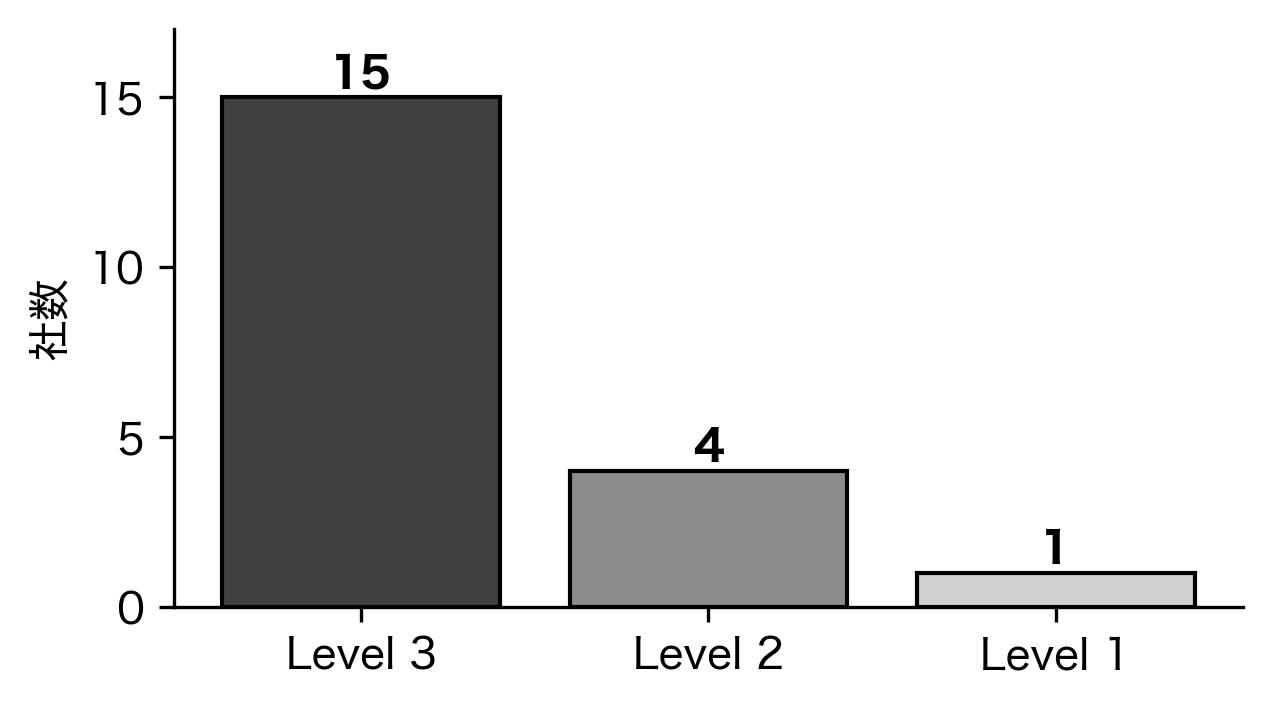
\includegraphics[width=0.55\linewidth]{p3_evidence_dist.png}
\caption{最終 20 社の Evidence Level 分布（L3：15 社，L2：4 社，L1：1 社）。}
\label{fig:evidence}
\end{figure}

Level 1 が 1 社残る（4350 メディカルシステムネットワーク）。同社は Phase1 の先行研究式（Value$\times$Quality）で選定された Buffett Core であり，Emerging の開示証拠を選定根拠にしていないため，Emerging 評価軸に対する低水準は選定妥当性を毀損しない。ただし事業継続性は一次資料で確認することを人間確認事項とする。なお Level 2 以上の判定は有価証券報告書・決算説明資料の個別精査（14 社）に依存しており，機械的スクリーニングでは Level 0〜1 までしか到達できない。この非対称性は\ref{sec:limits}節で限界として明記する。

% ---------- 7 ----------
\section{最終20社の役割設計}
\label{sec:roles}

最終 20 社は，完成した堀（Buffett Core）5・変わる堀（Transformation Core）5・生まれる堀（Emerging Core）5・両立型（Dual Moat）3・分散役（Bridge / Diversifier）2 の五役割で構成する。両立型は「Transformation が A/B 級または 60 点以上」かつ「Emerging が A/B 級かつ開示 Level 2 以上」を同時に満たす企業から選ぶ。集中を避けるため，同一業種は 3 社まで，同一テーマは 4 社まで（テーマ非依存を除く）とした。選定後に成績を見た入れ替えは一度も行っていない。

\begin{table}[H]
\caption{最終 20 社（役割別・正典 CSV より）}
\centering
\fontsize{8.7pt}{11pt}\selectfont
\begin{tabularx}{\linewidth}{p{34mm}Y}
\toprule
役割 & 銘柄（コード） \\
\midrule
完成した堀 5 & 3539 JM HD／4350 メディカルシステムN／6430 大黒電機／7803 ブシロード／9470 学研HD \\
変わる堀 5 & 5902 ホッカンHD／9828 元気グローバル／5233 太平洋セメント／8037 カメイ／3863 日本製紙 \\
生まれる堀 5 & 6368 オルガノ／6315 TOWA／6920 レーザーテック／6526 ソシオネクスト／5803 フジクラ \\
両立型 3 & 3697 SHIFT／6841 横河電機／9474 ゼンリン \\
分散役 2 & 3089 テクノアルファ／2112 塩水港精糖 \\
\bottomrule
\end{tabularx}
\end{table}

% ---------- 8 ----------
\section{除外862社の監査：反証可能性のために}
\label{sec:rejected}

選定の説明可能性は，選ばれた 20 社だけでなく，選ばれなかった側の記録で担保される。Top1200 のうち精査対象になった除外 862 社を，理由別にすべて記録した。

\begin{figure}[H]
\centering
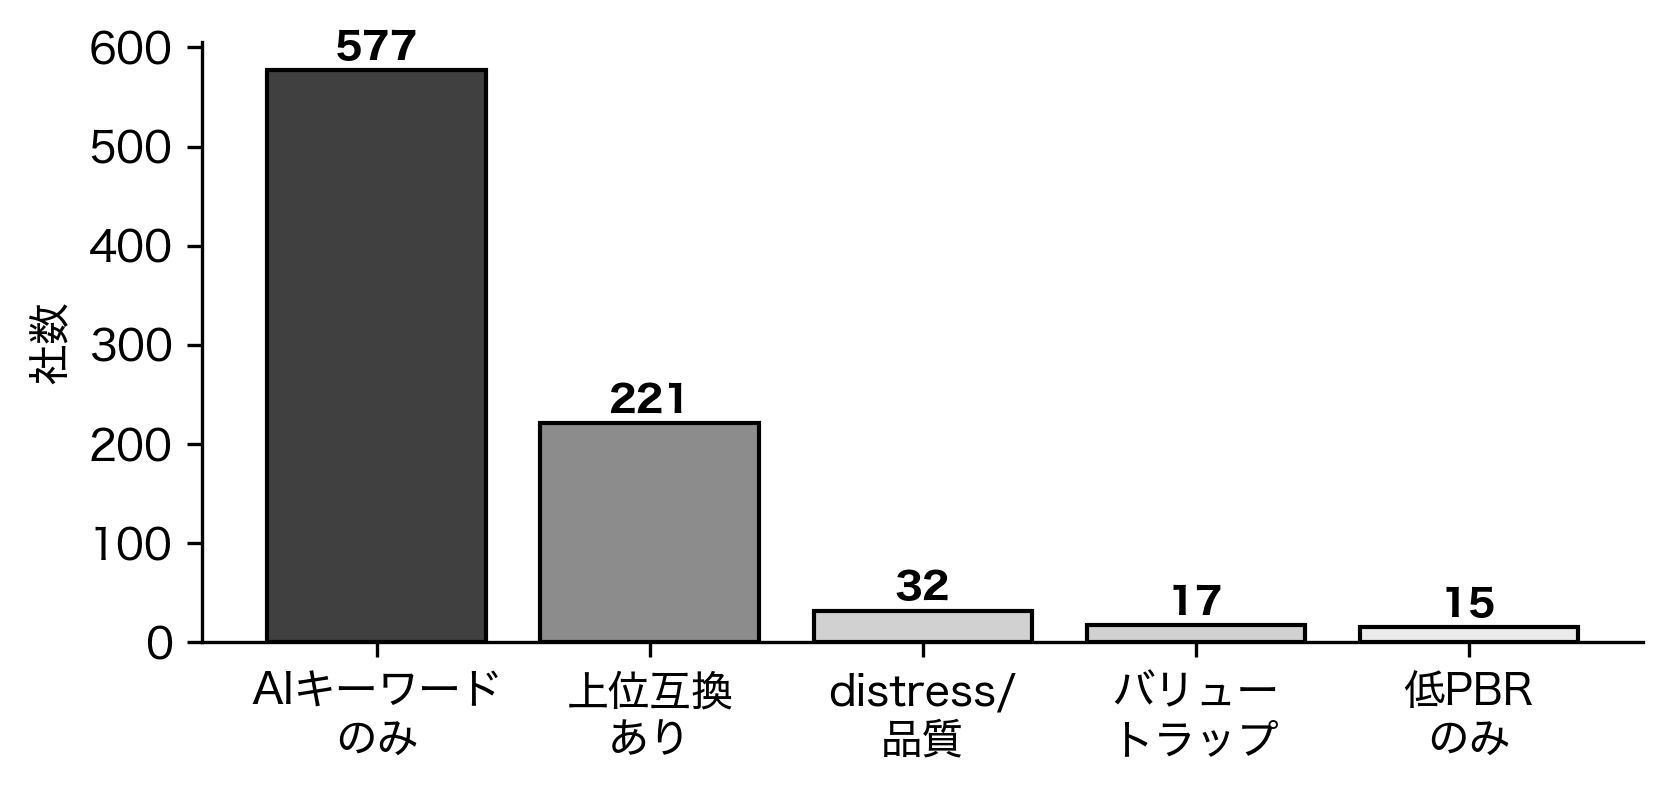
\includegraphics[width=0.8\linewidth]{p3_rejected.png}
\caption{除外 862 社の理由別内訳。AI キーワードのみが 577 社と圧倒的に多い。}
\label{fig:rejected}
\end{figure}

\begin{defbox}
「AI キーワードのみ 577 社」という数字は，生まれる堀の測定でもっとも重要な事実である。テーマに触れる企業は多いが，数量的裏づけを持つ企業は少ない。過熱ペナルティと証拠水準の分離がなければ，この 577 社がスコア上位に紛れ込む。
\end{defbox}

% ---------- 9 ----------
\section{頑健性：重みを動かしても選定は変わらないか}
\label{sec:robust}

式\eqref{eq:trans-partial}・\eqref{eq:emerging}の重みは，事後リターンで最適化した係数ではなく，概念上の設計係数である。恣意性への反論として，全重みを $\pm20\%$ 動かして再計算した。Top1200 の順位相関（Spearman $\rho$）は Transformation で最小 $0.997$，Emerging で最小 $0.994$ であり，選定される顔ぶれは変わらなかった。重みの微調整で結果を作っていないことの確認である。

% ---------- 10 ----------
\section{計算例：対照的な二社を0から評価する}
\label{sec:example}

正典データの実測値で，役割が分かれる仕組みを確かめる。

\begin{table}[H]
\caption{9470 学研 HD と 6368 オルガノの対比（実測値）}
\centering
\small
\begin{tabular}{lrrl}
\toprule
指標 & 9470 学研HD & 6368 オルガノ & 読み方 \\
\midrule
$\metric{BM}$（割安さ） & 1.526 & 0.167 & 学研は純資産の 1.5 倍，オルガノは市場評価が高い \\
Transformation & 73.4 & 66.9 & どちらも変わる堀の素質はある \\
Emerging & 21.5 & 74.3 & 生まれる堀はオルガノが圧倒的 \\
Evidence Level & L3 & L3 & どちらも数量根拠あり \\
役割 & 完成した堀 & 生まれる堀 & 学研は守 Top5 固定，オルガノは Emerging Core \\
\bottomrule
\end{tabular}
\end{table}

学研 HD は守の全関門を通過した完成した堀であり，Emerging が低くても役割上問題ない。オルガノは半導体向け超純水という実需（ボトルネック性・AI 基盤接続）が Emerging を押し上げ，生まれる堀の中核になる。一つのスコアで序列をつけるのではなく，役割ごとに適した物差しを当てる——これが三世代設計の要点である。

% ---------- 11 ----------
\section{限界と誠実な書き方}
\label{sec:limits}

\begin{itemize}
\item 設計完全形（式\eqref{eq:trans-design}）は選定に未使用である。株主還元・改革開示の構造化データ欠如により，partial 実装形（式\eqref{eq:trans-partial}）で運用した（partial 19 社・lite 1 社）。
\item 改革開示レベル（TR）は全対象で同値＝識別力ゼロであり，採用根拠に用いていない。
\item Emerging の Level 2 以上は 14 社の個別精査（curated）に依存する。精査していない企業が過小評価されている可能性がある。
\item 重みは設計係数であり，$\pm20\%$ 感度で選定不変を確認したが，最適性を主張するものではない。
\item スコアは将来リターンを予測しない。Phase3 は「証拠に裏づけられた構成」を作る段階であり，成果の検証は Phase5 の標本内確認に限られる。
\end{itemize}

\subsection{本文で使える要約文}
\begin{keybox}
Phase3 では，Phase2 の候補宇宙 Top1200 に対し，変わる堀（Transformation）と生まれる堀（Emerging）を測定した。Transformation は設計完全形ではなく，株主還元を FCF プロキシで代替した partial 実装形を選定に用いた（partial 19 社・lite 1 社）。Emerging はキーワードのみの 577 社を過熱ペナルティで除外し，証拠水準（Evidence Level）をスコアから分離して管理した。最終 20 社は完成・変化・新生の三世代 5/5/5 に両立型 3・分散役 2 を加えた五役割で構成し，除外 862 社を理由別に記録した。重みの $\pm20\%$ 感度で選定は不変であり，選定後に成績による入れ替えは行っていない。
\end{keybox}

% ---------- Appendix ----------
\newpage
\section{Appendix A：変数一覧}
\begin{longtable}{p{28mm}p{42mm}p{74mm}}
\caption{Phase3 で使う主な変数}\\
\toprule
記号 & 名称 & 意味 \\
\midrule
\endfirsthead
\toprule
記号 & 名称 & 意味 \\
\midrule
\endhead
$V_i$ & 評価ギャップ & B/M・E/P の正規化合成。割安の度合い。 \\
$C_i$ & 資本効率改善 & ROA 等の 3 年変化。改善の証拠。 \\
$R_i$ & 株主還元（設計） & 配当・自社株買い。データ欠如で未実装。 \\
$F_i$ & FCF プロキシ & $\metric{CFO}-\metric{CAPEX}>0$。還元余力の代理。 \\
$E_i$ & 改革開示（設計） & 経営改革の開示。識別力ゼロで除外。 \\
$X_i$ & 実行信頼性 & Piotroski available・CFO/NI。 \\
$Q_i$ & 利益の質 & Sloan・distress 安全度。 \\
$\Phi_i$ & Phase2 信頼度 & データの確からしさ（0〜1.1）。 \\
$P^{\mathrm{Trap}}_i$ & バリュートラップ罰 & 高アクルーアル・CF 赤字・継続損失。 \\
$I_i,N_i,B_i,A_i,D_i,T_i$ & Emerging 六要素 & 無形資産・技術・ボトルネック・AI 接続・顧客基盤・信頼安全。 \\
$B^{\mathrm{Evi}}_i$ & 証拠加点 & 開示証拠の強さ（最大 $+8$）。 \\
$P^{\mathrm{Hype}}_i$ & 過熱ペナルティ & キーワードのみは 18 点減点。 \\
$L^{TQ},L^{TS},L^{TR},L^{EM}$ & 証拠水準 & 定量・還元・改革・新興開示の各水準（0〜3）。 \\
$L^{\mathrm{final}}_i$ & 最終証拠水準 & 役割別に $\min/\max$ で決定（式\eqref{eq:evidence}）。 \\
\bottomrule
\end{longtable}

\section{References}
\begin{itemize}
\item Basu, S. (1977). Investment Performance of Common Stocks in Relation to Their Price-Earnings Ratios. \emph{Journal of Finance}, 32(3), 663--682.
\item Chan, L. K. C., Lakonishok, J., \& Sougiannis, T. (2001). The Stock Market Valuation of Research and Development Expenditures. \emph{Journal of Finance}, 56(6), 2431--2456.
\item Fama, E. F., \& French, K. R. (1993). Common Risk Factors in the Returns on Stocks and Bonds. \emph{Journal of Financial Economics}, 33(1), 3--56.
\item Lev, B., \& Gu, F. (2016). \emph{The End of Accounting and the Path Forward for Investors and Managers}. Wiley.
\item Novy-Marx, R. (2013). The Other Side of Value: The Gross Profitability Premium. \emph{Journal of Financial Economics}, 108(1), 1--28.
\item Peters, R. H., \& Taylor, L. A. (2017). Intangible Capital and the Investment-q Relation. \emph{Journal of Financial Economics}, 123(2), 251--272.
\item Piotroski, J. D. (2000). Value Investing. \emph{Journal of Accounting Research}, 38(Supplement), 1--41.
\item Sloan, R. G. (1996). Do Stock Prices Fully Reflect Information in Accruals and Cash Flows about Future Earnings? \emph{The Accounting Review}, 71(3), 289--315.
\item 経済産業省（2014）『伊藤レポート』．
\item 東京証券取引所（2023）「資本コストや株価を意識した経営の実現に向けた対応について」．
\end{itemize}

\end{document}
